This chapter deals with the Android operating system which becomes more popular with the time. Android platform is quite different from Java plaform. They use the same language for source code of applications and the build process is also similar but the differences cause that they are not fully compatible.

In Section~\ref{AndroidIntroduction}, Android and its history is presented. Architecture of this platform is described in Section~\ref{AndroidArchitecture} and part of this architecture -- Android runtime is discussed in more detail in Section~\ref{AndroidRuntime}. Basic components of Android application are presented in Section~\ref{AppStructure} and the build process of Android source code and resources is described in Section~\ref{buildProcess}

\section{Introduction}\label{AndroidIntroduction}
Android \cite{AndroidBook, AndroidProgBook} is a mobile operating system developed by Google. It's an open-source system based on the Linux kernel mainly used in mobile devices such as smartphones, tablets and smart watches but it can be found also in devices such as set-top boxes, media players and other electronics.

Android, Inc. was founded in California USA in 2003. Google, Inc. bought Android two years later. In 2007, Google acquired several patents in the field of mobile devices. At the same year on November 5, there is official presentation of an association of companies formed the Open Handset Alliance which aims to create open standards for mobile devices. The first smartphone running Android released on October 22, 2008.

Table \ref{androidHistory} presents a brief history of the Android operating system. It describes release dates of major versions, the numbering which change by the size of a system modifications, code names represented by a popular foods from version 1.5 and API levels in the last column.

\begin {table}[h!]
    \begin{tabular}{|l|c|l|c|}
    \hline
    {\bf Release date}  & {\bf Version} & {\bf Codename}        & {\bf API level}   \\
    \hline \hline
    September 23, 2008  & 1.0 -- 1.1    & ---                   & 1 -- 2            \\
    \hline
    April 27, 2009      & 1.5           & Cupcake               & 3                 \\
    \hline
    September 15, 2009  & 1.6           & Donut                 & 4                 \\
    \hline
    October 26, 2009    & 2.0 -- 2.1    & Eclair                & 5 -- 7            \\
    \hline
    May 20, 2010        & 2.2 -- 2.2.3  & Froyo                 & 8                 \\
    \hline
    December 6, 2010    & 2.3 -- 2.3.7  & Gingerbread           & 9 -- 10           \\
    \hline
    February 22, 2011   & 3.0 -- 3.2    & Honeycomb             & 11 -- 13          \\
    \hline
    October 18, 2011    & 4.0 -- 4.0.4  & Ice Cream Sandwich    & 14 -- 15          \\
    \hline
    July 9, 2012        & 4.1 -- 4.3    & Jelly Bean            & 16 -- 18          \\
    \hline
    October 31, 2013    & 4.4 -- 4.4.4  & KitKat                & 19 -- 20          \\
    \hline
    November 12, 2014   & 5.0 -- 5.0.2  & Lollipop              & 21                \\
    \hline
    \end{tabular}
    \centering
    \caption{Android version history}
    \label{androidHistory}
\end{table}

\section{Architecture}\label{AndroidArchitecture}
The following section describes the architecture of Android system \cite{AndroidDevBook} which consists from six layers. Figure~\ref{androidArchitecture} shows this architecture starting with kernel layer and ending with user application.

\paragraph{Linux kernel}
The lowest layer stands between hardware devices and other architecture layers. Android is based on a special version of the Linux kernel and several accessories such as memory management system, the Binder IPC driver and others. Since the beginning, Android was built on the Linux 2.6 kernel but the latest Android version runs on the kernel 3.4.

\paragraph{Hardware abstraction layer}
Hardware abstraction layer (HAL) is standart interface which allows Android system calls to drivers layer while he does not care what is the implementation of drivers and hardware in the lower layers. For each piece of hardware should be a driver and matching HAL providing hardware options.

\paragraph{Libraries}
Above the HAL is a layer of native libraries. These libraries are written in C or C ++ language and it can be accessed through the Android Standard Development Kit (SDK), but if direct access is required, it is possible to do that through the Native Development Kit (NDK). The HAL includes the following libraries:

\begin{itemize}
\item \textbf{Surface manager} -- library for composing different drawing surfaces windows on the screen
\item \textbf{Media Framework} -- provides various multimedia codecs for playing and recording video in many formats
\item \textbf{SQLite} -- a database engine for the use in data storage
\item \textbf{WebKit} -- a browser engine for displaying web content
\item \textbf{Libc} -- the standard library of the C programming language
\item \textbf{OpenGL ES} -- a library for support 2D and 3D graphics and hardware accelerated rendering
\item \textbf{Audio Manager} -- a library for working with sounds of device
\item \textbf{FreeType} -- a library for bitmap and vector font rendering
\item \textbf{SSL} -- a library for the use of encryption protocol for secure Internet communications
\end{itemize}

\paragraph{Android runtime}
Android runtime layer is located next to native libraries. This layer consist of two parts. The first one is the Core Libraries and the second one is the Dalvik Virtual Machine. The Core libraries can be further subdivided into two parts: Java Libraries and Android libraries.
\\
\begin{figure}[h!]
    \centering
    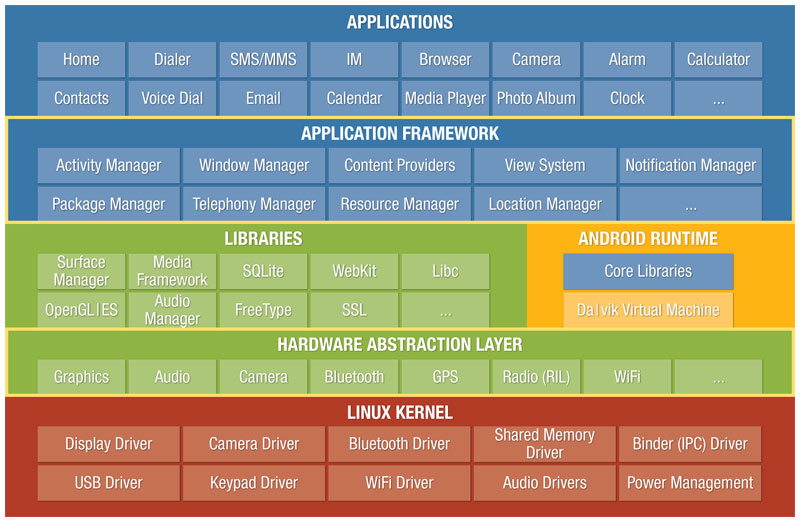
\includegraphics[scale=0.5]{fig/android_architecture.jpg}
    \caption{Android architecture \cite{AndroidArch}}
    \label{androidArchitecture}
\end{figure}

\paragraph{Application framework}
Application framework layer provides many high-level services to applications in the form of Java libraries. For developers, this is the most important layer that allows access to the device services. The Application framework includes the following parts:
 
\begin{itemize}
\item \textbf{Activity manager} -- controls all aspects of running activities. It manages all Services and Activities  described in Section~\ref{AppStructure}.
\item \textbf{Windows manager} -- provides services for windows management such as visibility and arrangement. It also takes care about animation on the screen.
\item \textbf{Content Providers} -- allows to work with the contents of other applications, it encapsulates the data, and provide mechanisms for defining data security.
\item \textbf{View System} -- a set of basic blocks that is used to build the application user interface. The basis of every graphical component is thr View class which is represented by a rectangular area on the screen.
\item \textbf{Notification manager} -- provides the possibility how to inform the user about some action that happened in the background. Notifications can take different forms like LED flashing, vibrating, ringing or notification on display.
\item \textbf{Package manager} -- allows obtaining of various information about applications that are currently installed on device.
\item \textbf{Telephony manager} -- provides access to telephone services of device. These services include SIM card, network, cellphone and other information.
\item \textbf{Resource manager} -- allows access to non-code resources such as color settings, layouts and strings. Separating of resources from code helps to better management of various characteristic withour modifying code.
\item \textbf{Location manager} -- provides access to the location services. These services allow periodical receiving of geographic coordinates and therefore it is possible to track device current location.
\end{itemize}

\paragraph{Applications}
The last and highest layer consists of the application itself. These comprise both pre-installed applications and applications that have been added over time from the Android store or an other way.

\section{Android runtime}\label{AndroidRuntime}
Both Android runtime and JRE include a virtual machine and Java SE API. In case of Android runtime, Android contains special virtual machine named Dalvik Virtual Machine and API lacks several Java packages and classes and contains special Android libraries.

\subsubsection{Dalvik Virtual Machine (DVM)}
DVM is a virtual machine that is being developed since 2005 and it was included into the system due to the JVM was not licensed as open-source in those times. The second reason was the optimization for mobile devices. 

Each application runs on an Android devices within its own instance of DVM (i.e. not as a process in the Linux kernel).

Running applications on a virtual machine has many advantages. First, it operates in a sandbox and thus can not interfere with the operating system or to other applications. Secondly, it makes the application platform independent and therefore can be run on any hardware. Advantages also include its DVM efficiency in memory usage and is thus better adaptation for use on mobile devices.

An application code must be always transformed from a standard \texttt{.java} file into bytecode but it is different from Java applications from this point. Bytecode is not executed by DVM but instead of bytecode it is converted by \texttt{dex} tool to Dalvik executables (\texttt{.dex} format). The whole process is described in the Section~\ref{buildProcess}.


\paragraph{Java libraries}
Most of Android applications are written using Java. Android contains libraries based on Apache Harmony Project that is an open-source Java implementation. These libraries are a subset of the Java SE platform. They do not contain all of the packages. For example \texttt{java.awt} or \texttt{java.swing} libraries are replaced by Android user interface classes and packages. More detailed comparison can be found in Chapter~\ref{apis}.

\paragraph{Android libraries}
Android libraries contain specific packages that provide all the functionality of Android devices. Libraries are written in Java and they includes the following packages:

\begin{itemize}
\item \textbf{android.app} -- provides access to the application model and it is the cornerstone of all applications
\item \textbf{android.content} -- classes for accessing and publishing data applications
\item \textbf{android.database} -- classes for data access and database manipulation 
\item \textbf{android.graphics} -- library for screen low-level 2D graphics drawing
\item \textbf{android.hardware} -- provide access to hardware features such as cameras and sensors
\item \textbf{android.media} -- library for handling with multimedia 
\item \textbf{android.text} -- library for manipulation and rendering of strings
\item \textbf{android.util} -- common tools such as data manipulation and time utils, conversions between numbers and strings, and other classes
\item \textbf{android.view} -- basic library for building a graphical user interface
\item \textbf{android.webkit} -- libraries for working with web content
\end{itemize}

\section{Application structure}\label{AppStructure}
In this section, anatomy of application is described. Application consist of the various components and blocks whose description follows.

\paragraph{Activities}
Activities represent one single screen of user interface. Typically after starting an application, the main activity shows and from there, another activity can be run or perform other operations. When you start a new activity, the previous one is stored in a LIFO stack. After pressing the back button, the stored Activity is invoked again.

\paragraph{Services}
Services are components that run in the background performing long-term tasks. They do not provide a user interface. Services may be still active in the background while other applications is running. For example, a service might be playing music or downloading from the Internet.

\paragraph{Content providers}
Content providers store, load data and make them available for other applications. Through the content providers other applications may modify or manipulate specific data. An example might be a content provider that manages the contact information on the device.

\paragraph{Intents}
Intents are messages between one component and other component. Intent can be sent to inside or outside of an application and that means one applications can communicate with other. The three types of application components are supported for Intents communication -- Activities, Services, and Broadcast receivers. There are two types of intents: Explicit and Implicit. Explicit intents specify the component to start by name. Implicit intents do not specify the component, another application can handle it and makes appropriate response.

\paragraph{Broadcast receivers}
These components are used to listen message notifications (Intents) from outside (other application or system) or from inside of the application. After receiving the message, receivers can initiate appropriate reaction. An example might be a incoming sms or low battery notification.

\paragraph{Application Resources}
Android application consists not only from Java files but also from the resources that are separated from the source code. These resources include:
\begin{itemize}
\item \textbf{Animation Resources} -- define predefined animation
\item \textbf{Color State List Resources} -- define color change based on the View state
\item \textbf{Drawable Resources} -- define different bitmaps or xml graphics files
\item \textbf{Layout Resources} -- define the layout of application components
\item \textbf{Menu Resources} -- define content of aplication menus
\item \textbf{String Resources} -- define string and string arrays
\item \textbf{Style Resources} -- define the appearance and format of ui elements.
\end{itemize}

\paragraph{Application manifest file}
Each application must have an \texttt{AndroidManifest.xml} file. This file contains information about application with regard to Android and it has to be placed in root directory of project. It must contains a unique package name for the application, the declaration of used Activity and Service components, application permissions to the protected parts of the API (such as access to the camera, etc.). There also have to be declared a minimum API level, list of connected and used libraries and other important informations about application. Android manifest is together with resources compiled by \texttt{aapt} tool to \texttt{R.java} file. Thanks to this, the information is then available in the source code.

\section{Build Process}\label{buildProcess}
Build process is the way how \texttt{.apk} package is produced from Android project. Apk file is a package file format used to distribution and installation of application software to Android devices. It contains all of the necessery files to run an application. Figure~\ref{buildProcess} shows how apk package is created from Java source code and resources, including Android Manifest file. The individual steps are:

\begin{enumerate}
\item The Android Asset Packaging Tool compiles resource files and \texttt{AndroidManifest.xml} and produce \texttt{R.java}. Resource references from Java code are then linked to this file.
\item \texttt{aidl} tool coverts all \texttt{.aidl} interfacese to Java interfaces. Aidl files are interfaces used for interprocess communication between client and service.
\item Java compiler takes and compiles \texttt{R.java} file, application source code and Java interfaces to bytecode. Bytecode is stored in \texttt{.class} output files. 
\item Any 3rd party libraries and \texttt{.class} files are converted by Dex tool to Dalvik byte code which is stored in \texttt{.dex} files.
\item Other uncompiled resource (eg. images), compiled resource and \texttt{.dex} files are processed by \texttt{apkbuilder} tool which packs them to \texttt{.apk} file.
\item Once the \texttt{.apk} is created, it must be signed by debug or release key. \texttt{jarsigner} tool provides signing and creates signed \texttt{.apk} file.
\item Finally, if the application is being signed in release mode, \texttt{zipalign} tool align the \texttt{.apk} file. It creates signed and aligned \texttt{.apk} file which is not so memory consuming.
\end{enumerate}

\begin{figure}[h!]
    \centering
    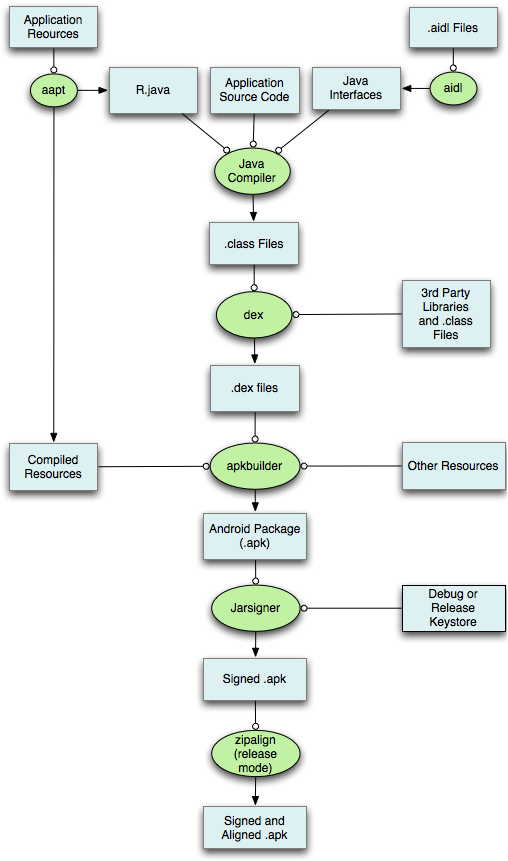
\includegraphics[scale=0.45]{fig/build.png}
    \caption{Build process \cite{AndroidDev}}
\end{figure}

